\documentclass[12pt,utf8,notheorems,compress,t]{beamer}
\usepackage{etex}
\usepackage[english]{babel}
\usepackage{tikz-cd}
\usepackage{mathtools}
\usepackage{booktabs}
\usepackage{array}
\usepackage{ragged2e}
\usepackage{multicol}
\usepackage{tabto}
\usepackage{xstring}
\usepackage{mathtools}
\usepackage{soul,xcolor}
%\setul{0.3ex}{}
\usepackage[all]{xy}
\xyoption{rotate}
\usepackage{tikz}
\usetikzlibrary{calc,shapes.callouts,shapes.arrows}
\usepackage{mathrsfs}
\hypersetup{colorlinks=true}

\usepackage[protrusion=true,expansion=true]{microtype}

\setlength\parskip{\medskipamount}
\setlength\parindent{0pt}

\title{Differenzielle Äquivariante $K$-Theorie}
\author{Eric Schlarmann}
\date{9. Juli 2020}

\usetheme{Warsaw}
\usecolortheme{seahorse}
%\usefonttheme{default}?
%\usepackage{kurier}?
\usefonttheme{serif}
\usepackage[T1]{fontenc}
\usepackage{libertine}
%\usepackage{mathpazo}
\useinnertheme{rectangles}

\newcommand{\A}{\mathcal{A}}
\renewcommand{\AA}{\mathbb{A}}
\newcommand{\E}{\mathcal{E}}
\newcommand{\F}{\mathcal{F}}
\renewcommand{\G}{\mathcal{G}}
\newcommand{\GG}{\mathbb{G}}
\renewcommand{\O}{\mathcal{O}}
\newcommand{\K}{\mathcal{K}}
\newcommand{\NN}{\mathbb{N}}
\newcommand{\RR}{\mathbb{R}}
\newcommand{\PP}{\mathbb{P}}
\newcommand{\ZZ}{\mathbb{Z}}
\renewcommand{\P}{\mathcal{P}}
\newcommand{\ppp}{\mathfrak{p}}
\newcommand{\defeq}{\vcentcolon=}
\newcommand{\defeqv}{\vcentcolon\equiv}
\newcommand{\Sh}{\mathrm{Sh}}
\newcommand{\GL}{\mathrm{GL}}
\newcommand{\Zar}{\mathrm{Zar}}
\newcommand{\op}{\mathrm{op}}
\newcommand{\Set}{\mathrm{Set}}
\newcommand{\Sch}{\mathrm{Sch}}
\newcommand{\LRS}{\mathrm{LRS}}
\newcommand{\Hom}{\mathrm{Hom}}
\DeclareMathOperator{\Spec}{Spec}
\newcommand{\lra}{\longrightarrow}
\newcommand{\RelSpec}{\operatorname{\text{\ul{$\mathrm{Spec}$}}}}
\renewcommand{\_}{\mathpunct{.}}
\newcommand{\?}{\,{:}\,}
\newcommand{\speak}[1]{\ulcorner\text{\textnormal{#1}}\urcorner}
\newcommand{\ull}[1]{\underline{#1}}
\newcommand{\affl}{\ensuremath{{\ull{\AA}^1_S}}}
\newcommand{\Ll}{\vcentcolon\!\Longleftrightarrow}
\newcommand{\dd}{\textup{d}} 
\newcommand{\reg}{\textup{reg}} 
\newcommand{\CC}{\mathbb{C}} 
%conflict
\newcommand{\R}{\mathbb{R}} 
\newcommand{\Q}{\mathbb{Q}} 
\newcommand{\Z}{\mathbb{Z}}
%\newcommand{\K}{\mathbb{K}}
\newcommand{\N}{\mathbb{N}}
\newcommand{\ci}{\textup{i}}
%\newcommand{\E}{\mathscr{E}}
\newcommand{\h}{\mathscr{H}}
%\newcommand{\G}{\mathscr{G}}
\newcommand{\tr}{\mathrm{tr}}
\newcommand{\ch}{\mathrm{ch}}
\newcommand{\Ch}{\mathrm{Ch}}
\newcommand{\CS}{\mathrm{CS}}
\newcommand{\grres}{\mathrm{Gr}_{\mathrm{res}}}
\newcommand{\glres}{\mathrm{GL}_{\mathrm{res}}}
\newcommand{\lglres}{\mathfrak{gl}_{\mathrm{res}}}
\newcommand{\fred}{\mathrm{Fred}}
\newcommand{\ff}{\mathscr{F}}
\newcommand{\bb}{\mathscr{B}}
\newcommand{\iu}{{i\mkern1mu}}

\setbeamertemplate{blocks}[rounded][shadow=false]

\newcommand{\fmini}[2]{\framebox{\begin{minipage}{#1}#2\end{minipage}}}
\makeatletter
\def\underunbrace#1{\mathop{\vtop{\m@th\ialign{##\crcr
      $\hfil\displaystyle{#1}\hfil$\crcr\noalign{\kern3\p@\nointerlineskip}
      \crcr\noalign{\kern3\p@}}}}\limits}
\def\overunbrace#1{\mathop{\vbox{\m@th\ialign{##\crcr\noalign{\kern3\p@}
      \crcr\noalign{\kern3\p@\nointerlineskip}
      $\hfil\displaystyle{#1}\hfil$\crcr}}}\limits}
\makeatother

\newenvironment{changemargin}[2]{%
  \begin{list}{}{%
    \setlength{\topsep}{0pt}%
    \setlength{\leftmargin}{#1}%
    \setlength{\rightmargin}{#2}%
    \setlength{\listparindent}{\parindent}%
    \setlength{\itemindent}{\parindent}%
    \setlength{\parsep}{\parskip}%
  }%
  \item[]}{\end{list}}

\newcommand{\pointthis}[2]{%
  \tikz[remember picture,baseline]{\node[anchor=base,inner sep=0,outer sep=0]%
    (#1) {#1};\node[overlay,rectangle callout,%
    callout relative pointer={(-0.5cm,0.8cm)},fill=blue!20] at
    ($(#1.north)+(1.1cm,-1.4cm)$) {#2};}%
}%

\newcommand{\hcancel}[5]{%
  \tikz[baseline=(tocancel.base)]{
    \node[inner sep=0pt,outer sep=0pt] (tocancel) {#1};
    \draw[red, line width=0.4mm] ($(tocancel.south west)+(#2,#3)$) --
    ($(tocancel.north east)+(#4,#5)$);
  }%
}

\newcommand{\slogan}[1]{%
  \begin{center}%
    \setlength{\fboxrule}{2pt}%
    \setlength{\fboxsep}{8pt}%
    {\usebeamercolor[fg]{item}\fbox{\usebeamercolor[fg]{normal text}\parbox{0.84\textwidth}{#1}}}%
  \end{center}%
}

\newcommand{\sloganwithoutborder}[1]{%
  \begin{center}%
    \setlength{\fboxrule}{0pt}%
    \setlength{\fboxsep}{-14pt}%
    {\usebeamercolor[fg]{item}\fbox{\usebeamercolor[fg]{normal
    text}\parbox{0.9\textwidth}{\begin{center}#1\end{center}}}}%
  \end{center}%
}


\setbeamertemplate{frametitle}[default][colsep=-2bp,rounded=false,shadow=false,center]

\setbeamertemplate{headline}{}
\setbeamertemplate{navigation symbols}{}

\newcounter{framenumberpreappendix}
\newcommand{\backupstart}{
  \setcounter{framenumberpreappendix}{\value{framenumber}}
}
\newcommand{\backupend}{
  \addtocounter{framenumberpreappendix}{-\value{framenumber}}
  \addtocounter{framenumber}{\value{framenumberpreappendix}} 
}

\setbeamertemplate{footline}{%
  \begin{beamercolorbox}[wd=\paperwidth,ht=2.5ex,dp=1.25ex,right,rightskip=1mm,leftskip=1mm]{frametitle right}
    {\quad} \inserttitle \hfill
    \insertframenumber\,/\,\inserttotalframenumber {\quad}
  \end{beamercolorbox}}

\newcommand{\hil}[1]{{\usebeamercolor[fg]{item}{\textbf{#1}}}}

\IfSubStr{\jobname}{\detokenize{nonotes}}{
  \setbeameroption{hide notes}
}{
  \setbeameroption{show notes}
}
\setbeamertemplate{note page}[plain]

\makeatletter
\let\ST\st
\renewcommand\st{%
    \let\set@color\beamerorig@set@color
    \let\reset@color\beamerorig@reset@color
    \ST}
\makeatother

\begin{document}

\addtocounter{framenumber}{-1}

\begin{frame}[c]
  \centering
  %\includegraphics[scale=0.3]{images/external-internal-small}
  \medskip

  \hil{Ein Kozykel-Modell für \\den äquivarianten Chern-Charakter und \\
  differenzielle äquivariante $K$-Theorie.}
%  \hil{A cocycle model for the equivariant \\Chern character and differential\\
%    equivariant K-theory}


%  \medskip
  \bigskip

  \scriptsize
  Eric Schlarmann\\[2em]
  \medskip
%  Regional Geometry and Topology Meeting\\
%  University of Regensburg and University of Augsburg \\
%  \ \\
  Dissertationsprüfung am \\[0.5em]
  9. Juli 2020
  \par
\end{frame}

%\backupstart
%\frame[t]{\frametitle{Outline}\scriptsize
%\begin{itemize}
%\item[]
%\tableofcontents
%\end{itemize}}
%\backupend 
\setstcolor{red}

%\begin{frame}\frametitle{Was ist Differenzielle $K$-Theorie?}
%    Als Geometer studieren wir glatte Mannigfaltigkeiten. Häufig nutzen wir
%    dabei Werkzeuge der Topologie.
%    \begin{minipage}{0.5\linewidth}
%        \vspace{1em}
%        \begin{itemize}
%            \item (Ko-)Homologietheorien
%            \item Homotopiegruppen
%            \item \dots
%        \end{itemize}
%    \end{minipage}
%    \begin{minipage}{0.4\linewidth}
%        \vspace{1.5em}
%        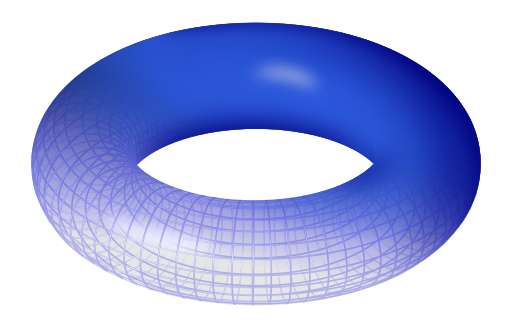
\includegraphics[scale=0.3]{512px-Torus}	
%    \end{minipage}
%    \vspace{1em} \vspace{1em}
%    \hil{Aber:} Glatte Struktur wird von diesen Werkzeugen ignoriert!
%\end{frame}
\begin{frame}\frametitle{Was ist Differenzielle $K$-Theorie?}
    \begin{block}{\onslide<2->{\textcolor{red}{Differenzielle}}
        Kohomologietheorien}
        Sind Familien von Funktoren Mfd $\rightarrow$ AbGrp mit Eigenschaften
       \begin{itemize}
           \item Mayer-Vietoris Sequenz
           \item $\coprod$ wird zu $\prod$
           \item
           \only<1>{Homotopieinvarianz}
           \only<2->{\hcancel{Homotopieinvarianz}{0pt}{3pt}{0pt}{-2pt}}
       \end{itemize}
    \end{block}\vspace{1em}
    \begin{exampleblock}{Beispiele}
    \begin{itemize}
            \item
                \only<1>{\hil{$H^*$:}}\only<2->{\hil{$\hat H^*$:}}
                \only<2->{Differenzielle} De Rham Kohomologie
            \item \only<1>{\hil{$K^*$:}}\only<2->{\hil{$\hat K^*$:}}
                \only<2->{Differenzielle} $K$-Theorie
      	    \item \only<1>{\hil{$MU^*$:}} \only<2->{\hil{$
		    \widehat {MU}^*$:}}
                \only<2->{Differenzieller} Komplexer Bordismus
	    \item \dots
    \end{itemize}
    \end{exampleblock}
\end{frame}
\begin{frame}\frametitle{Klassische Definition}
Für jede glatte Mannigfaltigkeit $M$ fordern wir ein kommutatives Diagram
\begin{equation}\begin{tikzcd}[ampersand replacement=\&]
        \textcolor{red}{\hat K^*(M)} \arrow[d,
        "R", red]\arrow[r, "I", red] \& K^*(M)\arrow[d, "\mathrm{ch}"] \\ 
        \Omega^*_{\dd=0}(M) \arrow[r, "\mathrm{Rham}"]\& H^*(M),
\end{tikzcd}\nonumber
\end{equation} \vspace{1em} sowie eine exakte Sequenz\vspace{-2em}
\begin{equation}\begin{tikzcd}[ampersand replacement=\&]
        K^{*-1}(M)\arrow[r, "\mathrm{ch}"]\&[-10pt]\Omega^{*-1}(M) /
        \mathrm{im}(\dd)\ar[dr, "\dd"]\arrow[r, "a", red] \&[-10pt]
        \textcolor{red}{\hat K^*(M)} \arrow[r, "I", red]\ar[d, "R", red]
        \&[-10pt] K^*(M) \arrow[r] \&[-10pt]  0 \\ \&\& \Omega^*_{\dd=0}(M)\&\&
\end{tikzcd}\nonumber
\end{equation}
\end{frame}
\begin{frame}{Äquivariantes Setting}

    Sei $G$ eine endliche Gruppe und $M$ eine $G$-Mannigfaltigkeit. Dann gibt es
    nach Atiyah und Segal eine äquivariante Version von $K$-Theorie.
    
    \textcolor{blue}{Motto:} Ersetze Vektorbündel durch äquivariante
    $G$-Vektorbündel!
    \vspace{1em}
    \begin{block}{Frage}
        Kann man die Axiome anpassen, um eine äquivariante Version der 
        \emph{differenziellen} K-Theorie definieren?
    \end{block}
\end{frame}

\begin{frame}\frametitle{Äquivariante Version, 1. Versuch}
\begin{equation}\begin{tikzcd}[ampersand replacement=\&]
        \textcolor{red}{\hat K_G^*(M)} \arrow[d,
        "R", red]\arrow[r, "I", red] \& K_G^*(M)\arrow[d, "\mathrm{ch}_G"] \\ 
        (\Omega^*_{\dd=0}(M))^G \arrow[r, "\mathrm{Rham}"]\& H_G^*(M),
\end{tikzcd}\nonumber
\end{equation}
wobei $\ch_G(E) = \ch(EG\times_G E \to EG\times_G M)$.
\vspace{0.5em} 

\onslide<2->{\hil{Aber:} Borel äquivariante Kohomologie ist kein gutes Ziel für
den Chern Charakter!}
\begin{block}<2->{Erinnerung:}
    Verkleben von $K$-Theorie Klassen mit Differenzialformen über den Chern
    Charakter. 
\end{block}
\end{frame}
\begin{frame}{Der Delokalisierte Chern Charakter}
    Nach Baum und Connes gibt es eine Möglichkeit, die (rationale)
    Isomorphieeigenschaft wieder herzustellen.
    \begin{block}{Delokalisierte Kohomologie}
        \vspace{-1em}
        \begin{align*}
            H^0_\mathrm{delok}(M) &= \left( \bigoplus_{g\in G} \prod_{k\in\N}
            H^{2k}(M^g;\CC)\right)^G\quad\mathrm{und}\\
            H^1_\mathrm{delok}(M) &= \left( \bigoplus_{g\in G} \prod_{k\in\N}
            H^{2k+1}(M^g;\CC)\right)^G.
        \end{align*}
        und es gibt einen Chern Charakter Isomorphismus
        \begin{align*}
            K_G^*(M)\otimes \CC
            \stackrel{\mathrm{ch}_{\mathrm{delok}}}{\longrightarrow}
            H_\mathrm{delok}^*(M)
        \end{align*}
    \end{block}
\end{frame}
\begin{frame}\frametitle{Äquivariante Version, 2. Versuch}
\begin{equation}\begin{tikzcd}[ampersand replacement=\&]
        \textcolor{red}{\hat K_G^*(M)} \arrow[d,
        "R", red]\arrow[r, "I", red] \& K_G^*(M)\arrow[d,
        "\mathrm{ch}_{\mathrm{delok}}"] \\ 
        \Omega^*_{\mathrm{delok}, \dd=0}(M) \arrow[r, "\mathrm{Rham}"]\&
        H_{\mathrm{delok}}^*(M)
\end{tikzcd}\nonumber
\end{equation}

\only<2->{Eine solche Theorie $\hat K_G^*$ würde wie im nicht äquivarianten
Fall den $K_G$-Theorie Funktor differenzialgeometrisch verfeinern!

Wie konstruiert man einen geeigneten Funktor $\hat K_G^*$?}
\end{frame}

\begin{frame}{$K$-Theorie über ein Spektrum}
    \begin{exampleblock}{Theorem (Atiyah)}{}
        \vspace{-1em}
        \begin{align*}
            K_G^0(M) &\cong [M, \mathscr{F}_0]_G \\
            K_G^1(M) &\cong [M, \mathscr{F}_1]_G,
        \end{align*}
        wobei $\mathscr{F}_i\subset \mathrm{Fred}(\mathcal{H}\otimes L^2(G))$
        geeignete Unterräume in der Norm Topologie mit Konjugationswirkung.
    \end{exampleblock}
    \onslide{\textcolor{blue}{Idee:} Die universellen Räume $\mathscr{F}_i$
        besitzen jeweils eine \emph{universelle} $K$-Theorie Klasse, welche wir
    entlang von Abbildungen zurückziehen. (``Indexbündel'')}
\end{frame}
\begin{frame}
    Eine differenzielle $K$-Theorie Klasse besteht aus
    \begin{itemize}
        \item einer $K$-Theorie Klasse $x$
        \item einem Differenzialform-Repräsentanten ihres Chern Charakters
            $\Ch(x)$.
    \end{itemize}
    \onslide<2->{Wenn wir einen universellen Repräsentanten für den Chern
    Charakter finden, können wir also möglicherweise differenzielle $K$-Theorie
    klassifizieren!
    
    Auf Atiyahs Räumen von Fredholm Operatoren sind bis heute allerdings keine
    konkreten geometrischen Repräsentanten bekannt.

    $\textcolor{blue}{\Rightarrow}$ Wir brauchen bessere Modelle von den
    klassifizierenden Räumen!}
    
\end{frame}
\begin{frame}
    Arbeiten von Segal, Quillen und Freed beschäftigen sich mit unendlich
    dimensionalen Mannigfaltigkeiten, um den universellen Chern Charakter zu
    beschreiben.
    \begin{block}<2->{Definition}
        Die eingeschränkte Grassmann Mannigfaltigkeit
        $\mathrm{Gr}_{\mathrm{res}}$ ist der Raum aller Unterräume $W\subset
        \mathcal{H}_+ \oplus \mathcal{H}_-$, sodass 
        \begin{itemize}
            \item $\pi_+\colon W\to \mathcal{H}_+$ ein Fredholm Operator ist.
            \item $\pi_-\colon W \to \mathcal{H}_-$ ein Hilbert--Schmidt
                Operator ist.
        \end{itemize}
    \end{block}
    \begin{block}<3->{Definition}
        Die eingeschränkte unitäre Gruppe $\mathrm U^1$ ist der Raum aller
        beschränkten
        unitären Operatoren $P$ auf $\mathcal{H}_+$, sodass $P-\mathrm{id}\in
        L^1$ ein Spurklasseoperator ist.
    \end{block}
\end{frame}

\begin{frame}{Klassifizierende Räume für $K$-Theorie}
    \begin{block}{Theorem}
        Für jede glatte $G$-Mannigfaltigkeit ist 
        \begin{align*}
            ([M, \mathrm{Gr}_{\mathrm{res}}]_G,\boxplus) &\cong K_G^0(M) \\
            ([M, \mathrm{U}^1]_G,\boxplus) &\cong K_G^1(M) \\
        \end{align*}
    \end{block}
    wobei die Blocksummenoperation
    \begin{align*}
        \boxplus\colon \grres \times \grres &\to \grres \\\boxplus\colon
        \mathrm U^1 \times \mathrm
        U^1 &\to \mathrm U^1,
    \end{align*}
    der Summe von Untervektorräumen bzw. Blocksumme von Matrizen entspricht.
\end{frame}
\begin{frame}
    Auf $\grres$ und $\mathrm U^1$ existieren (per Konstruktion!) spezielle
    Lie-Algebra-wertige Differenzialformen:
    \begin{itemize}
        \item Die Krümmungsform auf dem universellen Bündel $R\in
            \Omega^2(\mathrm{Gr}_{\mathrm{res}}; L^1)$.
        \item Die Maurer--Cartan Form $\omega\in \Omega^1(\mathrm U^1;
            L^1)$.
    \end{itemize}
    \begin{block}<2->{Theorem}
        Die folgenden Differenzialformen sind de Rham Repräsentanten des
        universellen delokalisierten Chern Charakters:
        \begin{align*}
            \ch_{\mathrm{even}} &= \bigoplus_{g\in G} \tr \left( g \exp\left(
            \frac{i}{2\pi}R_g \right) \right). \\
            \ch_{\mathrm{odd}} &= \bigoplus_{g\in G} \sum_{k\geq 1}
            \left(\frac{i}{2\pi}\right)^{k}
            \frac{(-1)^{k-1}(k-1)!}{(2k-1)!}\tr \left(g\,
            (\omega_g)^{2k-1}\right)
        \end{align*}
    \end{block}
\end{frame}

\begin{frame}{Äquivariante Differenzielle $K$-Theorie}
    \begin{block}{Definition/Theorem}
        Die Gruppen
        \begin{align*}
            \hat K_G^0(M) &= \textrm{Map}^G_{\mathrm{Smooth}}(M,
            \grres)\color<3->{red}{\times
            \Omega^1_{\mathrm{delok}}(M)} \color{black}{/\sim}\\
            \hat K_G^{1}(M) &= \textrm{Map}^G_{\mathrm{Smooth}}(M, \mathrm
            U^1)\color<3->{red}{\times\Omega^0_{\mathrm{delok}}(M)}
            \color{black}{/ \sim},
        \end{align*}
        definieren eine differenzielle Erweiterung. \onslide<2->{Hierbei ist
            $(f_1,\omega_1) \sim (f_0,\omega_0)$, 
        falls es eine glatte $G$-Homotopie $f_t$ von $f_0$ zu $f_1$ gibt, sodass
        \begin{align*}
            \CS_G(f_t) = \bigoplus_g \int_I \Ch(f_t) = \omega_1 - \omega_0 +
            \mathrm{exakt} 
        \end{align*}}
    \end{block}
\end{frame}
\begin{frame}
    \begin{block}{Vermutung (Äquivariantes Venice-Lemma)}
        Sei
        \begin{align*}
            \dd\omega\in \Omega^0_{\mathrm{delok}}(M) \qquad \mathrm{oder} \qquad
            \dd\omega\in \Omega^1_{\mathrm{delok}}(M)
        \end{align*}
        eine exakte delokalisierte Differenzialform. Dann ist $\dd \omega$ die
        Chern Form $f^*\ch$ einer nullhomotopen $G$-Abbildung
        \begin{align*}
            f\colon M \to
            \mathrm{Gr}_{\mathrm{res}}\quad \mathrm{oder}\quad f\colon M
            \to\mathrm U^1.
        \end{align*}
    \end{block}
    Wenn das äquivariante Venice-Lemma gilt, so kann man stets auf Zykel
    $(f,\omega)$ mit $\omega=0$ reduzieren. Somit ist in diesem Fall jede Klasse
    in $\hat K_G$ allein durch eine Abbildung $f$ charakterisiert.
\end{frame}
\begin{frame}{Zykelabbildungen (gerader Fall)}
    Ein Zykel für $K_G^0(M)$ ist ein $G$-Vektorbündel $E\to M$. Es
    gibt eine natürliche Transformation
    \begin{align*}
        \mathrm{cycl}\colon \mathrm{Vect}_G\to K_G^0,
    \end{align*}
    die wir die \emph{topologische Zykelabbildung} nennen.

    Ein \hil{geometrischer Lift} der topologischen Zykelabbildung ist eine natürliche
    Transformation
    \begin{align*}
        \widehat{\mathrm{cycl}}\colon \mathrm{Vect}^{\nabla}_G\to \hat K_G^0,
    \end{align*}
    mit $R\circ \widehat{\mathrm{cycl}} = \mathrm{Ch}_G$ und $I\circ
    \widehat{\mathrm{cycl}} = \mathrm{cycl}$.
\end{frame}
\begin{frame}
    Zykelabbildungen sind nützlich, um Klassen in $\hat K_G$ explizit zu
    beschreiben!
    \begin{block}{Theorem (Existenz von Zykelabbildungen)}
            Die oben definierte differenzielle Erweiterung $\hat K_G^*$ besitzt
            sowohl eine gerade als auch eine ungerade geometrische Zykelabbildung.
    \end{block}
    \begin{block}{Theorem (Äquivariante Eindeutigkeit)}
        Bis auf Isomorphie ist $\hat K_G^*$ die eindeutige differenzielle
        Erweiterung, die sowohl eine gerade, als auch eine ungerade
        Zykelabbildung zulässt. 
    \end{block}
\end{frame}
\begin{frame}\frametitle{Offene Fragen}
    \begin{itemize}
        \item Kompakte Lie Gruppen / diskrete Gruppen?
        \item Explizite Cup Produkt Struktur auf $\hat K_G$?
        \item Explizite Pushforward / Indexabbildungen?
        \item Erweiterung auf unendlich-dimensionale Mannigfaltigkeiten?
        \item Mehr explizite Berechnungen!
    \end{itemize}
    \vspace{2em}\centering\hil{Vielen Dank für eure Aufmerksamkeit!}
\end{frame}
\end{document}
